\documentclass[a4paper,10pt]{article}
\usepackage[utf8]{inputenc}
\usepackage{graphicx}
\usepackage{url}

%opening
\title{Assignment 1: CS 763, Computer Vision}
\author{}

\begin{document}

\maketitle

You are given two datasets. The file names are Features2D\_dataset1.mat, Features3D\_dataset1.mat,
Features2D\_dataset2.mat and \\ Features3D\_dataset2.mat. Each dataset contains (1) the XYZ coordinates 
of $N$ points marked out on a calibration object, and (2) the XY coordinates of their corresponding projections
onto an image plane.Your job is to write a MATLAB program which will determine the $3 \times 4$ projection
matrix $M$ such that $P_1 = MP$ where $P$ is a $4 \times N$ matrix containing the 3D object points
(in homogeneous coordinates) and $P_1$ is a $3 \times N$ matrix containing the image points (in homogeneous 
coordinates). Use the SVD method and print out the matrix $M$ on screen (include it in your pdf file as well). 
Write a piece of code to verify that your computed $M$ is correct. For any one dataset, repeat the computation
of the matrix $M$ after adding zero mean i.i.d. Gaussian noise of standard deviation $\sigma = 0.05 \times max_c$ (where $max_c$ is the maximum 
absolute value of the X,Y,Z coordinate) to every coordinate of $P$ and $P_1$ (leave the homogeneous coordinates unchanged). Comment on your results. Include these 
comments in your pdf file that you will submit. \textbf{Tips:} A mat file can be loaded into MATLAB memory using the `load' command. To add Gaussian noise, 
use the command `randn'.

The MATLAB code is enclosed in the zip file.
We calculated the M for both datasets.
\\for dataset1:

$M$ = \[ \left( \begin{array}{cccc}
		-0.2905 & -0.0532 & 0.1866 & 0.6283\\
		0.0881 & -0.3264 & 0.0881 & 0.6010\\
		-0.0002 & -0.0002 & -0.0002 & 0.0021\\
              \end{array} \right)\] 
for dataset2:

$M$ = \[ \left( \begin{array}{cccc}
		-0.0087 & -0.0011  & 0.0039 & -0.9986\\
		-0.0001 & -0.0092 & -0.0005 &  0.0520\\
		-0.0000 & -0.0000 & -0.0000 & -0.0027\\
              \end{array} \right)\]

We added Gaussian noise by using \textbf{randn} function to each points in dataset1. After this step M was found to be

$M$ = \[ \left( \begin{array}{cccc}
    0.3024  & 0.0480 & -0.1855 & -0.6297\\
   -0.0817  & 0.3209 & -0.0929 & -0.5975\\
    0.0002  & 0.0002 &  0.0002 & -0.0021\\
              \end{array} \right)\]
              
Before Adding noise we had got the first point in 2D using $MP$ as 
$P$ = \[ \left( \begin{array}{cc}
               300.5 & 574.0207\\
              \end{array} \right)\]
Which is very near if not exactly same as the given 2D point. But after adding noise $P$ became
$P$ = \[ \left( \begin{array}{cc}
               301.1632 & 573.0596\\
              \end{array} \right)\]

              
Hence we can see that the eror in estimating the correct correspondence in the points might lead to error in 
calibration matrix.\\
\\
In this exercise, you will estimate the homography between a pair of images using the method we studied in class. 
You should use the well-known SIFT algorithm to (1) detect salient feature points in both the images, 
and (2) determine pairs of matching points given the two point sets (`matching point pair' refers to points in 
the two images representing the same physical entity). The code for performing both these tasks is available at 
\url{http://www.cs.ubc.ca/~lowe/keypoints/}. We may study the internal details of how SIFT works in a separate set
of lectures in class, but for this exercise, just assume this package is a magic blackbox. Now, given this set of
matching pairs of points produced by the SIFT package, your job is to estimate the homography between the point 
sets. Write a routine of the form $\textrm{H = homography(im1,im2)}$ where $H$ is the homography matrix that will
transform the first image. You will use data from the folder \url{http://www.cse.iitb.ac.in/~ajitvr/CS763_Spring2015/HW1/Homography/}. Do as follows:

\begin{enumerate}
\item Apply the homography transformation in the file `Hmodel.mat' to the image `goi1\_downsampled.jpg' using
reverse warping to generate a warped image. Now estimate the homography that transforms the first image into 
its warped version. Apply the estimated transformation to the first image (using reverse warping) and display 
all three images side by side in your report. Also print the model and estimated homography matrices (make sure
you normalize both so that $H(3,3) = 1$ in both cases). 
\item Determine the homography that transforms the image `goi1\_downsampled.jpg' to the second image
`goi2\_downsampled.jpg'. Warp the first image (using reverse warping) and compare it to the second. Display all 
three images side by side in your report. Also print the estimated homography matrix normalized so that 
$H(3,3) = 1$. 
\end{enumerate}

In the first part transformation in 'Hmodel.mat' is \\
$Hmodel$ = \[ \left( \begin{array}{cccc}
    1.1283 &  0.0385 & -57.1714\\
    0.0702 &  1.0931 & -40.8860\\
    0.0005 &  0.0002 &  1.0000\\
              \end{array} \right)\]
and transformation got from Homography is

$homographyTransform$ = \[ \left( \begin{array}{cccc}
    1.3241 &  0.0891 & -82.1921\\
    0.1917 &  1.2541 & -72.5790\\
    0.0003 &  0.0001 &  1.0000\\
              \end{array} \right)\]
            
            
Figure1 shows the effect of the above transformation to the images. First image is the original image,
second is the image transformed by $Hmodel$ transformation given in 'Hmodel.mat' file and third image is the image 
got from transforming the original image using transformation got from Homography(Given by $homographyTransform$).
\\
\\
\begin{figure}[ht!]
\centering
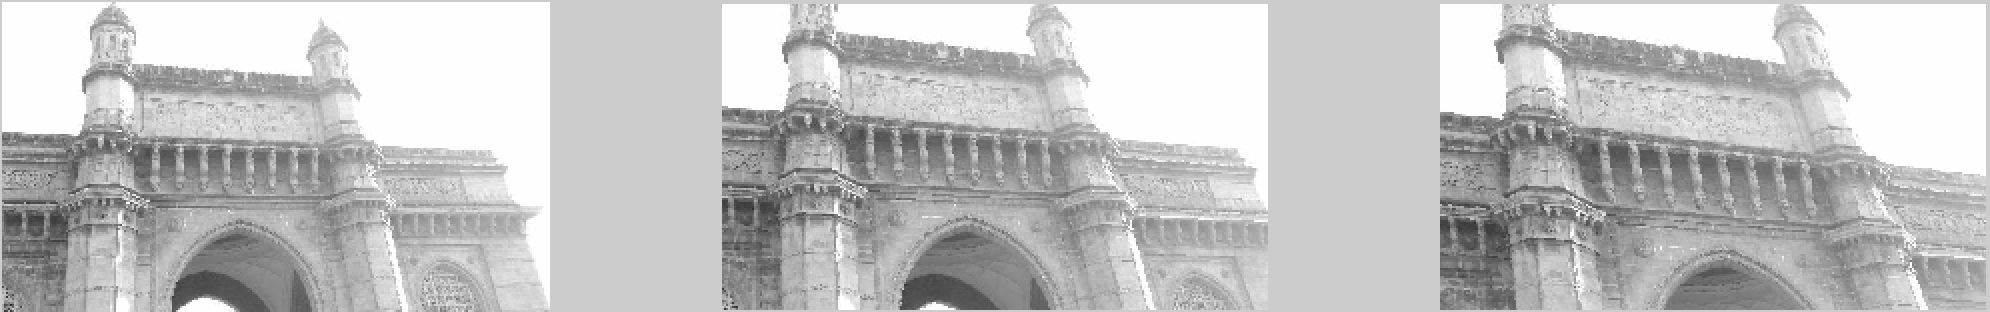
\includegraphics[width=90mm]{figure1.png}
\caption{}
\end{figure}

In the second part homography transform is 

    $homographyTransform$ = \[ \left( \begin{array}{cccc}
    0.9279 & -0.0650 & 34.1957\\
   -0.0359 &  0.8910 & 49.5626\\
   -0.0001 & -0.0002 &  1.0000\\
             \end{array} \right)\]       

Figure shows the results. First image is the original image, second is the image got from ‘goi2 downsampled.jpg’
and third is the image got from transforming the original image using the transformation got from Homography (Given by $homographyTransform$)
\begin{figure}[ht!]
\centering
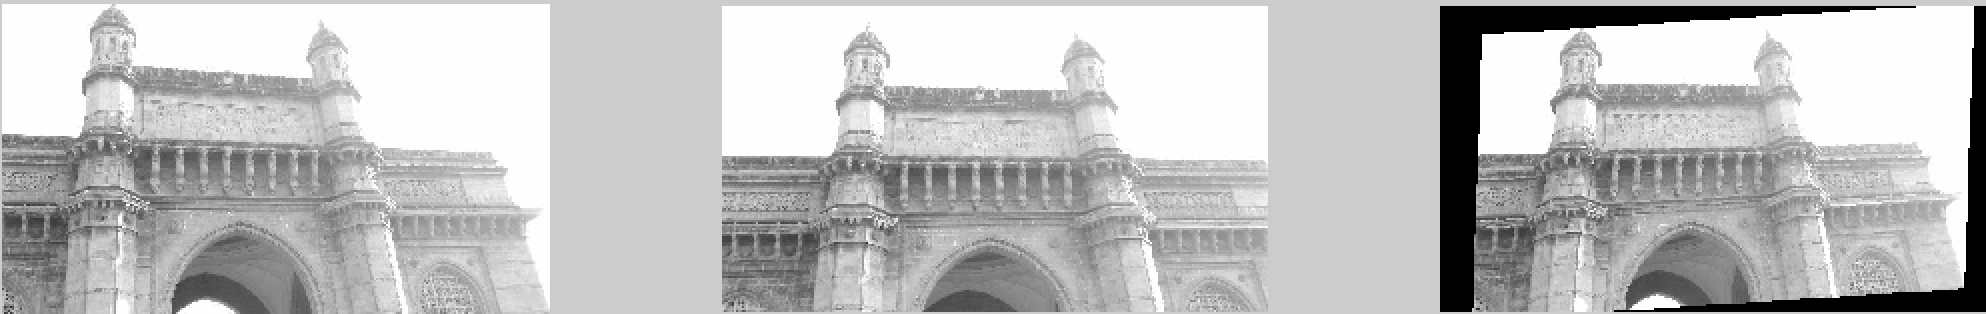
\includegraphics[width=90mm]{figure2.png}
\caption{}
\end{figure}

\end{document}
